\documentclass[aspectratio=169,t,13pt,usenames,dvipsnames]{beamer}
\usetheme[lily]{PaloAlto}
\usecolortheme{dolphin}
\usepackage{mathtools}
\usepackage{lmodern}
\usepackage{tikz}
\usepackage{pgfplots}
\usepackage{tikz-3dplot}
\usepackage{adjustbox}
\usetikzlibrary{quantikz}
\usepackage{xcolor}
\usepackage{bm}
\pgfplotsset{compat=newest}
\logo{%
\stackbox[c][c]{
\includegraphics[height=1.15cm]{logo.pdf}\\[-3pt]{\textcopyright~2021}\\{Ron K. Cytron}}}

% \logo{
\includegraphics[height=2.5cm]{logo.pdf}}
\def\ColorR#1{\textcolor{BrickRed}{#1}}
\def\ColorG#1{\textcolor{\RCthree}{#1}}
\def\ColorB#1{\textcolor{\RCtwo}{#1}}
\definecolor{links}{HTML}{2E8B57}
\hypersetup{colorlinks,linkcolor=,urlcolor=links}
%%
%% From stackoverflow
%%
\newcommand{\MyArrow}[1][0.1pt]{\tikz[baseline=-0.26em,y=3em, x=3em]{\filldraw[line width=#1] (0.4202,0.0021) .. controls (0.4202,-0.0000) and (0.4188,-0.0018) .. (0.4171,-0.0025) .. controls (0.3917,-0.0092) and (0.3699,-0.0236) .. (0.3509,-0.0401) .. controls (0.3355,-0.0538) and (0.3225,-0.0704) .. (0.3130,-0.0890) .. controls (0.3119,-0.0915) and (0.3094,-0.0929) .. (0.3066,-0.0929) .. controls (0.3028,-0.0929) and (0.2996,-0.0897) .. (0.2996,-0.0858) .. controls (0.2996,-0.0848) and (0.3000,-0.0837) .. (0.3003,-0.0827) .. controls (0.3087,-0.0665) and (0.3193,-0.0517) .. (0.3316,-0.0391) -- (0.1181,-0.0391) .. controls (0.1143,-0.0391) and (0.1111,-0.0359) .. (0.1111,-0.0320) .. controls (0.1111,-0.0282) and (0.1143,-0.0250) .. (0.1181,-0.0250) -- (0.3471,-0.0250) .. controls (0.3611,-0.0137) and (0.3766,-0.0046) .. (0.3935,0.0021) .. controls (0.3766,0.0088) and (0.3611,0.0179) .. (0.3471,0.0292) -- (0.1181,0.0292) .. controls (0.1143,0.0292) and (0.1111,0.0323) .. (0.1111,0.0362) .. controls (0.1111,0.0401) and (0.1143,0.0432) .. (0.1181,0.0432) -- (0.3316,0.0432) .. controls (0.3193,0.0559) and (0.3087,0.0707) .. (0.3003,0.0868) .. controls (0.3000,0.0879) and (0.2996,0.0889) .. (0.2996,0.0900) .. controls (0.2996,0.0939) and (0.3028,0.0970) .. (0.3066,0.0970) .. controls (0.3094,0.0970) and (0.3119,0.0956) .. (0.3130,0.0932) .. controls (0.3225,0.0745) and (0.3355,0.0580) .. (0.3509,0.0443) .. controls (0.3699,0.0278) and (0.3917,0.0133) .. (0.4171,0.0067) .. controls (0.4188,0.0059) and (0.4202,0.0042) .. (0.4202,0.0021) -- cycle;}}
\def\LinkArrow#1{%
\mbox{$\,$\href{#1}{\mbox{\vrule width 0pt height 0ex depth 0pt$\MyArrow[0.75pt]$}}}$\,$}
\def\WLOG{WLOG}
\def\True{\mbox{\texttt{True}}}
\def\False{\mbox{\texttt{False}}}
\def\Zero{\mbox{$0$}}
\def\One{\mbox{$1$}}
\def\Not#1{%
\ensuremath{\Overline{\ensuremath{#1}}}}
\def\Xor#1#2{\ensuremath{#1\oplus #2}}
\def\Nand#1#2{%
\ensuremath{\mbox{Nand}(#1,#2)}}
\def\And#1#2{%
\ensuremath{#1 \wedge #2}}
\def\Or#1#2{%
\ensuremath{#1 \vee #2}}
\def\Conj#1{%
\ensuremath{#1^{\star}}}
\def\Star#1{%
\Conj{#1}}
\def\EmptyString{\ensuremath{\lambda}}
\def\Mag#1{%
\ensuremath{{|\,#1\,|}}}
\def\PNorm#1#2{\ensuremath{\Mag{\kern-2pt\Mag{#1}\kern-2pt}}_{#2}}
\def\Prob#1{%
\ensuremath{\Mag{#1}^{2}}}
\def\CNOT#1#2{%
\ensuremath{\NamedGate{CNOT}(#1,#2)}}
\def\CNOTMatrix{%
\begin{pmatrix*}[r]
1 & 0 & 0 & 0 \\
0 & 1 & 0 & 0 \\
0 & 0 & 0 & 1 \\
0 & 0 & 1 & 0\end{pmatrix*}%
}
\def\CCNOT#1#2#3{%
\ensuremath{\mbox{\NamedGate{CNOT}}(#1,#2,#3)}}
\long\def\ToDo#1{\smash{\textcolor{YellowOrange}{#1}}}
\def\ApplyGate#1#2{%
\ensuremath{#1\,#2}}
\def\Inverse#1{\ensuremath{{#1}^{-1}}}
\def\Quote#1{``#1''}
\def\NamedGate#1{%
\mbox{\bfseries{\textrm{#1}}}}
\def\Identity{\NamedGate{I}}
\def\Hadamard{\NamedGate{H}}
\def\PauliX{\NamedGate{X}}
\def\PauliY{\NamedGate{Y}}
\def\PauliZ{\NamedGate{Z}}
\def\SQBG#1#2#3#4#5{%
\ensuremath{%
#1 \begin{pmatrix*}[r] #2 & #3 \\ #4 & #5\end{pmatrix*}}}
\def\HMatrix{%
\SQBG{\RootTwo{}}{1}{1}{1}{-1}}
\def\XMatrix{%
\SQBG{\relax}{0}{1}{1}{0}}
\def\ZMatrix{%
\SQBG{\relax}{1}{0}{0}{-1}}
\def\YMatrix{%
\SQBG{\relax}{0}{-i}{i}{0}}
\def\IMatrix{%
\SQBG{\relax}{1}{0}{0}{1}}
\def\Co#1{\mathbb{C}}
\def\Implies#1#2{\ensuremath{#1 \rightarrow\ #2}}
\def\Domain#1{\ensuremath{\mathcal{#1}}}
\def\CompClass#1{\Domain{#1}}
\def\SpecialX#1{\ensuremath{#1^{\star}}}
\def\Forall#1#2{\ensuremath{\forall\ #1, #2}}
\def\Degrees#1{\ensuremath{#1^{\circ}}}
\def\RootTwo{\ensuremath{\frac{1}{\sqrt{2}}}}
\def\TwoSupOp#1#2#3{%
\ensuremath{\RootTwo{}\left(#1 #3 #2\right)}}
\def\TwoSup#1#2{%
   \TwoSupOp{\ket{#1}}{\ket{#2}}{+}}
\def\QPlus{\TwoSupOp{\QZero}{\QOne}{+}}
\def\QMinus{\TwoSupOp{\QZero}{\QOne}{-}}
\def\Set#1{\ensuremath{\left\{\,#1\,\right\}}}
\def\BigSkip{%

\bigskip

}

\def\MedSkip{%

\medskip

}
\def\SmallSkip{%

\smallskip

}
\def\SineWave#1{%
{%
\pgfmathsetmacro{\Xone}{#1}
\pgfmathsetmacro{\Xtwo}{-(#1)}
\draw (0,0) sin(1,\Xone) cos (2,0) sin(3,\Xtwo) cos (4,0);
}
}
\newcommand{\tolstrut}{%
  \vrule height\dimexpr\fontcharht\font`\A+.1ex\relax width 0pt\relax
}

\DeclareRobustCommand{\Overline}[1]{%
  \ensuremath{\overline{\raisebox{0pt}[1.07\height]{#1}}}%
}
\newenvironment{TIKZP}[1][scale=1.0]{%
\adjustbox{valign=t}\bgroup
\begin{tikzpicture}[#1]
}{%
\end{tikzpicture}
\egroup
}
\long\def\Definition#1{%
\begin{block}{Definition}
#1
\end{block}}
\long\def\Postulate#1#2{%
\begin{block}{Postulate}
\begin{description} \item[#1] #2\end{description}
\end{block}}
\long\def\TwoUnequalColumns#1#2#3#4{%
\begin{columns}%
\begin{column}{#1}#3\end{column}%
\begin{column}{#2}#4\end{column}%
\end{columns}%
}
\long\def\ThreeUnequalColumns#1#2#3#4#5#6{%
\begin{columns}%
\begin{column}{#1}#4\end{column}%
\begin{column}{#2}#5\end{column}%
\begin{column}{#3}#6\end{column}%
\end{columns}%
}
\long\def\ThreeColumns#1#2#3{%
\ThreeUnequalColumns{0.33\textwidth}{0.33\textwidth}{0.33\textwidth}{#1}{#2}{#3}%
}
\long\def\TwoColumns#1#2{%
\TwoUnequalColumns{0.5\textwidth}{0.5\textwidth}{#1}{#2}%
}
\long\def\OnlyRemark#1#2{%
\only<#1>{\Remark{#2}}}

\long\def\Remark#1{%
\begin{block}{Remark}
#1
\end{block}}
\long\def\Example#1{%
\begin{example} #1\end{example}}
\def\VV{\textit{vice versa}}
\def\QZero{\ket{\hbox to 0.7em{\hss \ensuremath{0}\hss}}}
\def\QOne{\ket{\hbox to 0.7em{\hss \ensuremath{1}\hss}}}
\def\QState#1{\ket{\QName{#1}}}
\def\QName#1{\ensuremath{\psi_{#1}}}
\def\TensOp{\ensuremath{\bm{\otimes}}}
\def\TensProd#1#2{\ensuremath{#1 \TensOp{} #2}}
\def\TensSupProd#1#2{\ensuremath{#1^{\bm{\otimes} #2}}}
\def\PZero{\SQB{1}{0}}
\def\POne{\SQB{0}{1}}
\def\PPlus{\ensuremath{\RootTwo{}\SQB{1}{1}}}
\def\PMinus{\ensuremath{\RootTwo{}\SQB{1}{-1}}}
\def\PHad{\ensuremath\frac{1}{\sqrt{2}}\SQB{1}{1}}
\def\PHadm{\ensuremath\frac{1}{\sqrt{2}}\SQB{1}{-1}}
\def\Intersect#1#2{\ensuremath{#1 \cap #2}}
\def\Union#1#2{\ensuremath{#1 \cup #2}}
\def\Set#1{\ensuremath{\left\{\,#1\,\right\}}}
\def\BinAlph#1{\ensuremath{\Set{0,1}^{#1}}}
\def\AllBits#1#2{\ensuremath{#1\in \BinAlph{#2}}}
\def\DQB#1#2#3#4{%
\ensuremath{\begin{pmatrix*}[r] #1 \\ #2 \\ #3 \\ #4\end{pmatrix*}}}
\def\QQB#1#2#3#4#5#6#7#8{%
\ensuremath{\begin{pmatrix*}[r] #1 \\ #2 \\ #3 \\ #4 \\ #5 \\ #6 \\ #7 \\ #8\end{pmatrix*}}}
\def\SQB#1#2{%
\ensuremath{\begin{pmatrix*}[r] #1 \\ #2\end{pmatrix*}}}
\def\CQB#1#2{%
\ensuremath{\begin{pmatrix*}[r] #1 #2\end{pmatrix*}}}
\def\CDQB#1#2#3#4{%
\ensuremath{\begin{pmatrix*}[r] #1 #2 #3 #4\end{pmatrix*}}}
\def\TZPointDiam{2pt}
\def\TZPoint#1#2#3{%
\draw[fill=black] (#1) circle (\TZPointDiam) node[#3] {#2} ;}
\def\UnitComplexCircle{%
\draw [<->] (-1.5, 0) -- (1.5, 0)  node[right] {$\Re{}$} ;
   \draw [<->] (0,-1.5) -- (0, 1.5) node[above] {$\Im{}$} ;

   \draw (0, 0) circle (1) ;
   }
   \def\TZPEast{\TZPoint{1,0}{$+1$}{above right}}
   \def\TZPNorth{\TZPoint{0,1}{$\NiceI{}$}{above right}}
   \def\TZPWest{\TZPoint{-1,0}{$-1$}{above left}}
   \def\TZPSouth{\TZPoint{0,-1}{$-\NiceI{}$}{below right}}
\def\TZText#1#2#3{%
  \draw (#1) node [#3] {#2};
}
\def\Qiskit{\texttt{qiskit}}
\def\TwoToThe#1{\ensuremath{2^{#1}}}
\def\Exp#1{\ensuremath{e^{#1}}}
\def\NiceI{\kern 0.5pt\ensuremath{\mathfrak{i}}}
\def\ExpPhase#1{\Exp{\,\NiceI\,#1}}
\def\ExpNegPhase#1{\Exp{-\NiceI\,#1}}
%%
%% Not sure this is used
%%
\def\PhaseLabel#1{\phase{\fbox{#1}}}
%%
\def\ColHead#1{\begin{center}\bf #1\end{center}}
\def\Complex#1#2{\ComplexGen{#1}{#2}{+}}
\def\ComplexDiff#1#2{\ComplexGen{#1}{#2}{-}}
\def\ImaginaryM#1{\ComplexDiff{\relax}{#1}}
\def\ComplexGen#1#2#3{%
\ensuremath{#1 #3 i\relax #2}}
\def\Polar#1#2{\ensuremath{#1\hbox to 0.1pt{\hss}\Exp{\NiceI\relax#2}}}
%%
%% #1 -- lower left x
%% #2 -- lower left y
%% #3 -- upper right x
%% #4 -- upper right y
%% #5 -- num lines
\def\PFilter#1#2#3#4#5{

    \draw (#1,#2) -- (#3,#2) -- (#3,#4) -- (#1,#4) -- cycle;
    \foreach \i in {1,...,#5}
    {
        \pgfmathsetmacro{\PFilterInc}{#1 + (#3-#1) / #5 * \i}
        % \edef\PFilterInc{\pgfmathresult}
        \draw (\PFilterInc, #2) -- (\PFilterInc, #4);
    }
}
%% #1 - x
%% #2 - y
%% #3 - degrees
%% #4 - options
%% #5 - radius
\def\RadiantArrowsR#1#2#3{%
\foreach \p in {0, #1,...,360} {
   \draw[#2] (0,0)  -- (\p:#3) ;
}
}
\def\RadiantArrows#1#2{%
   \RadiantArrowsR{#1}{#2}{1}
}
\newcommand\RotateTheta[1][scale=1.0]{%
\SquareOutline{}
\begin{scope}[#1]
\fill[white] (0.5,0.5) circle (0.5);
\draw (0.5,0.5) circle (0.5);
\draw[->] (1.0,0.5) arc(0:45:0.5);
\draw (0.5,0.5) node {$\theta$};
\end{scope}
}
\def\SquareOutline{%
\path (0,0) rectangle (1,1);%
}%
\newcommand\Qif[1][scale=1.0]{%
\begin{scope}[#1]
\SquareOutline{}
\clip (0,0) rectangle(1,1);
\RotateAroundCenter{45}{%
\begin{scope}
\draw (0.15,0.15) rectangle(0.85,0.85);
\end{scope}}
\end{scope}
}
\newcommand\LightSource[1][scale=1.0]{%
\begin{scope}[#1]
\SquareOutline{}
\PhotonGun{}
\begin{scope}[shift={(0.75,0.5)}]
    \RadiantArrowsR{22.5}{color=red}{0.25}
\end{scope}
\end{scope}
}
\def\PhotonGun{%
\fill (0,0.375) rectangle (0.5, 0.625);
}
\def\HPolar{%
\begin{scope}[color=red]
\SquareOutline{}
\draw[thick] (0.5,0.4) -- ++(0.35,0)
             ++(-0.35,0.1) -- ++(0.35,0)
             ++(-0.35,0.1) -- ++(0.35,0);
% \fill (0.90,0.5) circle (0.05);
\end{scope}
}
\def\VPolar{%
\begin{scope}[color=red]
\draw[thick] (0.6,0.375) -- ++(0,.250)
             ++(0.1,-.250) -- ++(0,.250)
             ++(0.1,-.250) -- ++(0,.250);
% \fill (0.95,0.5) circle (0.05);
\end{scope}
}
\newcommand\HPolarizedLightSource[1][scale=1.0]{%
\begin{scope}[#1]
\SquareOutline{}
\PhotonGun{}
\HPolar{}
\end{scope}
}
\newcommand\VPolarizedLightSource[1][scale=1.0]{%
\begin{scope}[#1]
\SquareOutline{}
\PhotonGun{}
\VPolar{}
\end{scope}
}
\newcommand\EVBomb[1][scale=1.0]{%
\begin{scope}[#1]
\fill (0.5,0.5) circle(0.5);
\end{scope}%
}
\newcommand\EVBoom[1][scale=1.0]{%
\begin{scope}[#1]
\fill[white] (0.5,0.5) circle(0.5);
\draw[red,thick] (0.5,0.5) circle(0.5);
\clip (0,0) rectangle(1,1);
\begin{scope}
\node[scale=0.35,xshift=28pt,yshift=28pt,starburst,draw,red,fill=orange,line width=1.5pt]
{BOOM!};
\end{scope}
\end{scope}
}
\newcommand\Measurement[1][scale=1.0]{%
\begin{scope}[#1]
\draw[color=white] (0,0) rectangle(1,1);
\begin{scope}
\clip (0.25,0.25) rectangle (1,1);
\draw (0,0) circle(0.9);
\draw (0,0) circle(1.0);
\end{scope}
\draw[thick] (0,0) --(0,1);
\draw[->] (0.25,0.25) -- (0.9,0.9);
\end{scope}
}
\def\TRectangle#1#2#3#4#5#6{%
\begin{scope}[#6]
\draw [fill=#5] (#1,#2) rectangle (#3,#4);
\end{scope}
}
%% #1 -- llx
%% #2 -- lly
%% #3 -- urx
%% #4 -- ury
%% #5 -- angle
\newcommand\Mirror[1][rotate=0]{%
\clip (0,0) rectangle(1,1);
\begin{scope}[#1]
   \SquareOutline{}
   \TRectangle{0}{.4375}{1}{.5625}{Gray}{rotate=0}
\end{scope}
}
\newcommand\BeamSplitter[1][scale=1.0]{%
\begin{scope}[#1]
    \SquareOutline{}
    \TRectangle{0}{.375}{1}{.625}{SkyBlue}{rotate=0}
\end{scope}
}
\def\MZ{%
\LightSource{}
\Shift{2}{0}{\RotateAroundCenter{-45}{\BeamSplitter{}}}
\Shift{2}{-2}{\RotateAroundCenter{-45}{\Mirror{}}}
\Shift{6}{0}{\RotateAroundCenter{-45}{\Mirror{}}}
\Shift{6}{-2}{\RotateAroundCenter{-45}{\BeamSplitter{}}}
\Shift{8}{-2}{\Measurement[color=orange]{}}
\Shift{6}{-4}{\RotateAroundCenter{-90}{\Measurement[color=\RCtwo]{}}}
}
\def\Shift#1#2#3{%
\begin{scope}[shift={(#1,#2)}] #3\end{scope}
}
\def\RotateAroundCenter#1#2{%
\begin{scope}[rotate around={#1:(0.5,0.5)}]
  #2
\end{scope}
}
\def\Vskip#1{\mbox{}\vskip #1\mbox{}}
\def\Hskip#1{\mbox{}\hskip #1\mbox{}}
\author{Ron K.~Cytron}
\institute{Washington University\\Saint Louis, Missouri\\[2em] \textcopyright~2021 All rights reserved by the author}
\setbeamertemplate{footline}[frame number]{}
%\setbeamertemplate{footline}[text line]{%
%  \parbox{\linewidth}{\vspace*{-8pt}\textcopyright~2021\hfill\insertshortauthor\hfill\insertpagenumber}}
%% #1 -- lecture number
%% #2 -- lecture title
%% #3 -- lecture subtitle
%% #4 -- lecture label
\def\SetTitle#1#2#3#4{%
   \title{#2}%
   \subtitle{#3}%
   \date{\today}%
   %\begin{frame}\maketitle\end{frame}%
   \frame{\titlepage}%
   \lecture[#1]{#2: #3}{lec:#4}%
}
\def\Kaye{\href{https://dl.acm.org/doi/10.5555/1206629}{Kaye}}
\def\MikeIke{\href{https://dl.acm.org/doi/10.5555/1972505}{Nielson~and~Chuang}}

\newcounter{ProtocolDialogStep}
\newenvironment{ProtocolDialog}[3]{%
\def\Incr{\stepcounter{ProtocolDialogStep}}
\def\Ref##1{\Incr{}\ThreeUnequalColumns{#1}{#2}{#3}{\arabic{ProtocolDialogStep}. ##1}{\relax}{\relax}}%
\def\Alice##1{\Incr{}\ThreeUnequalColumns{#1}{#2}{#3}{\relax}{\arabic{ProtocolDialogStep}. ##1}{\relax}}%
\def\All##1##2##3{%
\Incr{}
\ThreeUnequalColumns{#1}{#2}{#3}{\arabic{ProtocolDialogStep}. ##1}{##2}{##3}
}
\def\Bob##1{\Incr{}\ThreeUnequalColumns{#1}{#2}{#3}{\relax}{\relax}{
\arabic{ProtocolDialogStep}. ##1}}%
\setcounter{ProtocolDialogStep}{0}%
\ThreeUnequalColumns{#1}{#2}{#3}{\textbf{Ref}}{\textbf{Alice}}{\textbf{Bob}}
}{%
}
%% #1 -- options
%% #2 -- width
%% #3 -- height
%% #4 -- signals
\newenvironment{GateBox}[4][scale=1.0]{%
\edef\Signals{#4}%
\edef\Height{#3}%
\edef\Width{#2}%
\pgfmathsetmacro{\Max}{\Signals}%
\pgfmathsetmacro{\Vsep}{\Height / \Max}%
\pgfmathsetmacro{\Wlen}{\Width / 5}%
\def\ComputeMyY##1{%
   \pgfmathsetmacro{\MyY}{\Height - 0.5 * \Vsep - ##1*\Vsep}}%
\def\Input##1##2{%
   \pgfmathsetmacro{\Xone}{-\Wlen}
   \pgfmathsetmacro{\Xtwo}{0}
   \pgfmathsetmacro{\MyY}{\Height - 0.5 * \Vsep - ##1*\Vsep}
   \draw[->] (\Xone,\MyY) node[left] {##2} -- (\Xtwo,\MyY);
}%
\def\Output##1##2{%
   \pgfmathsetmacro{\Xone}{\Width}
   \pgfmathsetmacro{\Xtwo}{\Width + \Wlen}
   \pgfmathsetmacro{\MyY}{\Height - 0.5 * \Vsep - ##1*\Vsep}
   \draw[->] (\Xone,\MyY) -- (\Xtwo,\MyY) node[right] {##2};
}%
\def\BoxLabel##1{%
\node[draw, fit={(0,0) (\Width,\Height)}, inner sep=0pt, label=center:\mbox{##1}] (A) {};
}%
\begin{TIKZP}[#1]
   \draw (0,0) rectangle(#2,#3);
}{%
\end{TIKZP}}
%%
%% 1 options
%% 2 width
%% 3 height
%% 4 number of qubits
%%
\newenvironment{DotPBox}[4][scale=1.0]{%
\edef\Qubits{#4}%
\edef\Height{#3}%
\edef\Width{#2}%
\pgfmathsetmacro{\Max}{\Qubits}%
\pgfmathsetmacro{\Hsep}{\Width / \Max}%
\def\Qbit##1##2{%
   \pgfmathsetmacro{\MyX}{##1*\Hsep}
   \draw (\MyX,0) rectangle ++(\Hsep,\Height) node[pos=0.5] {\ensuremath{##2}};
}%
\begin{TIKZP}[#1]
}{%
\end{TIKZP}}
\def\PhiTheta#1#2{%
\mbox{\ensuremath{\textcolor{\RCone}{\phi = #1}, \textcolor{\RCtwo}{\theta = #2}}}}
%
% #2 -- orcacle name
% #3 -- upper left input
% #4 -- lower left input
% #5 -- upper right output
% #6 -- lower right output
%
\newenvironment{Oracle}[6][scale=1.0]{%
\begin{GateBox}[#1]{2.5}{1.5}{2}
\BoxLabel{#2}
\Input{0}{#3}
\Input{1}{#4}
\Output{0}{#5}
\Output{1}{#6}
}{%
\end{GateBox}
}
\newenvironment{TTable}[3]{%
\def\TRow##1##2##3{%
##1 & ##2 & ##3 \\}
\begin{tabular}{c|cc}
\TRow{#1}{#2}{#3}\hline
}{%
\end{tabular}
}
%%
%%  1 name
%%  2 one x
%%  3 one f(x)
%%  4 another x
%%  5 another f(x)
\def\SBitTable#1#2#3#4#5{%
\begin{center}
    \begin{TTable}{#1}{$x$}{$f(x)$}
    \TRow{ }{#2}{#3}
    \TRow{ }{#4}{#5}
    \end{TTable}
\end{center}}
%%
%%
\newenvironment{UTable}[6]{%
\def\URow##1##2##3##4##5##6{%
##1 & ##2 & ##3  & ##4 & ##5 & ##6\\}
\begin{tabular}{c|cc|c|cc}
& \multicolumn{2}{|c|}{Inputs} &
& \multicolumn{2}{|c}{Outputs} \\
\URow{#1}{#2}{#3}{#4}{#5}{#6}\hline
}{%
\end{tabular}
}
%%
%%  1 name
%%  2 one x
%%  3 one f(x)
%%  4 another x
%%  5 another f(x)
\def\SBitTable#1#2#3#4#5{%
\begin{center}
    \begin{TTable}{#1}{$x$}{$f(x)$}
    \TRow{ }{#2}{#3}
    \TRow{ }{#4}{#5}
    \end{TTable}
\end{center}}

\newenvironment{BlochSphere}[3][scale=1.0]{
    \bgroup%
    \def\BlochSpherePhiTheta{%
    \tdplotsetrotatedcoords{0}{0}{0};O
        \path[tdplot_rotated_coords] (1.0,0,0) arc (0:115:1.0) node(phi) {};
        \draw[tdplot_rotated_coords,thick,\RCone] (0.3,0,0) arc (0:115:0.3);
        \draw[tdplot_rotated_coords,\RCone,thick,dashed] (0,0,0) -- (phi);
        \draw[\RCone] (0.4,0.4,0) node {$\phi$};
        
        \tdplotsetrotatedcoords{25}{-90}{0};
        \path[tdplot_rotated_coords] (1,0,0) arc (0:45:1) node(theta) {};
        \draw[tdplot_rotated_coords,thick,\RCtwo] (0.4,0,0) arc (0:45:0.4);
        \draw[tdplot_rotated_coords,\RCtwo,thick] (0,0,0) -- (theta);
        \draw[\RCtwo] (-0.4,0,0.3) node {$\theta$};
        
        
    }
    \def\TZPointDiam{0.7pt}%
    \def\ShowAxes{%
    \draw[dashed, tdplot_rotated_coords, black] (1,0,0) node {{\Large\bf x}} (0,1,0) node {{\Large\bf y}} (0,0,1) node {{\Large\bf z}};
    }%
    \tdplotsetmaincoords{#2}{#3}%
    \begin{tikzpicture}[tdplot_main_coords, #1]
        
        
        \shade[ball color = lightgray, opacity = 0.5] (0,0,0) circle (1cm);
        
        %%
        %% The equator
        %%
        \tdplotsetrotatedcoords{0}{0}{0};
        \draw[dashed, tdplot_rotated_coords, gray] (0,0,0) circle (1);
        
        %%
        %% Arc in the x-z plane
        %%
        \tdplotsetrotatedcoords{90}{90}{90};
        \draw[dashed, tdplot_rotated_coords, gray] (1,0,0) arc (0:180:1);
        
        %%
        %% Arc in the y-z plane
        %%
        \tdplotsetrotatedcoords{0}{90}{90};
        \draw[dashed, tdplot_rotated_coords, gray] (1,0,0) arc (0:180:1);
        
        %\tdplotsetrotatedcoords{90}{90}{90};
       % \draw[dashed, tdplot_rotated_coords, black] (1,0,0) node {{\Large\bf x}} (0,1,0) node {{\Large\bf y}} (0,0,1) node {{\Large\bf z}}; 
        
        \draw[dashed, gray] (0,0,0) -- (-1,0,0);
        \draw[dashed, gray] (0,0,0) -- (0,-1,0);
        \draw[dashed, gray] (0,0,0) -- (0,0,-1);
        
        \draw[-stealth] (0,0,0) -- (1.30,0,0);
        \draw (1.45,0,0) node {$x$};
        \draw[-stealth] (0,0,0) -- (0,1.30,0);
        \draw(0,1.45,0) node {$y$};
        \draw[-stealth] (0,0,0) -- (0,0,1.30);
        \draw (0,0,1.45) node {$z$};
        
}{%
    \end{tikzpicture}
    \tdplotsetmaincoords{0}{0}
    \egroup
}

\long\def\Exercise#1#2{%
\relax}
\newcommand\QEDsym[1][2em]{\hbox to #1{\hss\ensuremath{\square}}}
\def\QED{\begin{flushright}\ensuremath{\square}\end{flushright}}
\def\UGateA{%
\ensuremath{\cos(\theta/2)}}
\def\UGateB{%
\ensuremath{-\ExpPhase{\lambda}\sin(\theta/2)}}
\def\UGateC{%
\ensuremath{\ExpPhase{\phi}\sin(\theta/2)}}
\def\UGateD{%
\ensuremath{\ExpPhase{(\phi+\lambda)}\cos(\theta/2)}}
\def\UGate{%
\SQBG{\relax}{\UGateA{}}{\UGateB{}}{\UGateC{}}{\UGateD{}}}%
\def\FCirc#1{%
\begin{tikzpicture}[scale=#1]%
\SquareOutline{}%
\fill (0.5,0.5) circle(0.4);%
\end{tikzpicture}%
}%
\def\SCirc{\FCirc{0.3}}%
\newenvironment{BBKey}[0]{%
\def\STD{%

\begin{tikzpicture}[scale=0.35]%
\SquareOutline{}%
\draw[ultra thick,purple] (0,0.5) -- (1,0.5);%
\draw[ultra thick,purple] (0.5,0) -- (0.5,1);%
\end{tikzpicture}}%
\def\HDM{%

\begin{tikzpicture}[scale=0.30]%
\SquareOutline{}%
\draw[ultra thick,purple] (0,0) -- (1,1);%
\draw[ultra thick,purple] (0,1) -- (1,0);%
\end{tikzpicture}}%
\def\BBUp{%

\begin{tikzpicture}[scale=0.30]%
\SquareOutline{}%
\draw[->,thick,purple] (0.5,0) -- (0.5,1);%
\end{tikzpicture}}%
\def\BBRt{%

\begin{tikzpicture}[scale=0.30]%
\SquareOutline{}%
\draw[->,thick,purple] (0,0.5) -- (1,0.5);%
\end{tikzpicture}}%
\def\BBNe{%

\begin{tikzpicture}[scale=0.30]%
\SquareOutline{}%
\draw[->,thick,purple] (0,0) -- (1,1);%
\end{tikzpicture}}%
\def\BBSe{%

\begin{tikzpicture}[scale=0.30]%
\SquareOutline{}%
\draw[->,thick,purple] (0,1) -- (1,0);%
\end{tikzpicture}}%
\def\BBBasis{%
\begin{tabular}{c|c|c}
Basis & 0 & 1 \\
\hline
\STD{} & \BBUp{} & \BBRt{} \\
\HDM{} & \BBNe{} & \BBSe{}
\end{tabular}%
}%
}{%
\relax%
}
\def\CFCirc#1{%
  \textcolor{#1}{\FCirc{0.30}}}
\def\Agree{%
  \textcolor{green}{\FCirc{0.30}}}%
\def\DisAgree{%
   \textcolor{red}{\FCirc{0.30}}}%
\def\MetaAgree{%
   \textcolor{yellow}{\FCirc{0.30}}}%
\newenvironment{EKey}[0]{%
\def\ZZ{%
\ZRot{0}%
}%
\def\ZZPO##1{%
\ZRot{\frac{\pi}{##1}}%
}%
\def\ZZNPO##1{%
\ZRot{\ensuremath{\,-\frac{\pi}{##1}}}%
}%
\def\ZRot##1{%
\ensuremath{Z_{##1}}%
}%
}{%
}
\def\AltAlert#1#2#3{%
\alt<#1>{\alert{#2}}{#3}}
\def\RCone{Rhodamine}
\def\RCtwo{CornflowerBlue}
\def\RCthree{LimeGreen}
\def\RCfour{Tan}
\def\RCfive{Plum}
\def\ColorOne#1{\textcolor{\RCone}{#1}}
\def\ColorTwo#1{\textcolor{\RCtwo}{#1}}
\def\ColorThree#1{\textcolor{\RCthree}{#1}}
\def\ColorFour#1{\textcolor{\RCfour}{#1}}
\def\ColorFive#1{\textcolor{\RCfive}{#1}}
\def\ColorBlack#1{\textcolor{black}{#1}}
\def\NegF#1{\NegOneExp{f(#1)}}
\def\NegOneExp#1{\ensuremath{(-1)^{#1}}}
\def\RootTwoN#1{\ensuremath{\frac{1}{\sqrt{2^{#1}}}}}
%%
%% var, exponent
%%
\def\SumBV#1#2{\OpBV{#1}{#2}{\displaystyle\sum\limits}}
\def\OpBV#1#2#3{\ensuremath{#3_{\AllBits{#1}{#2}}}}
\def\DotP#1#2{\ensuremath{#1\boldsymbol{\cdot}#2}}
\def\SumPH#1#2{\displaystyle\sum\limits_{#1=0}^{2^{#2}-1}}
%
% for hadamard results
%
%% #1 w for H((w>)
%% #2 free variable name
%% #3 n
\newcounter{HTableCounter}
\newenvironment{HTable}[3]{%
%% ##1 v^w
%% ##2 v . w
%% ##3 result
%% ##4 basis vector 000 001 etc.
\def\TE##1##2##3##4{%
\ensuremath{##4} & \ensuremath{##1} & \ensuremath{##2} & \ensuremath{##3 1} \ensuremath{\ket{##4}}}%
\begin{tabular}{c|c|c|r}
\multicolumn{4}{c}{$\sqrt{2^{#3}}$\,\Hadamard(\ket{#1})} \\ 
$v$ & \And{v}{#1} & \DotP{v}{#1} &  \multicolumn{1}{|c}{Term} \\ \hline}{%
\end{tabular}
}

\newcounter{ScrollCounter}
\newcounter{ScrollCounterEnd}
\newcounter{ScrollEOne}
\newcounter{ScrollETwo}
\newcounter{ScrollEThree}
\newcounter{ScrollEFour}
%%
%% start
%%
\newenvironment{ScrollingProof}[1][1]{%
   \setcounter{ScrollCounter}{#1}%
   \setcounter{ScrollEOne}{#1}%
   \setcounter{ScrollETwo}{#1}%
      \stepcounter{ScrollETwo}%
   \setcounter{ScrollEThree}{#1}%
      \stepcounter{ScrollEThree}\stepcounter{ScrollEThree}%
   \setcounter{ScrollEFour}{#1}%
      \stepcounter{ScrollEFour}\stepcounter{ScrollEFour}\stepcounter{ScrollEFour}
   \def\Curr{\value{ScrollCounter}}%
   \def\One{\value{ScrollEOne}}%
   \def\Two{\value{ScrollETwo}}%
   \def\Three{\value{ScrollEThree}}%
   \def\Four{\value{ScrollEFour}}%
   %\def\Memo##1{\gdef\RCScrollMemoText{##1}##1}
   %\def\Recall{\RCScrollMemoText}
   \def\Next##1##2{%
       \visible<\value{ScrollCounter}-##1>{##2}%
       %\def\Last{##2}%
    \stepcounter{ScrollCounter}%
    \stepcounter{ScrollEOne}%
    \stepcounter{ScrollETwo}%
    \stepcounter{ScrollEThree}%
    }%
    \def\Last##1{%
        \gdef\ScrollingLastText{##1}%
        \Next{\Two}{\visible<\value{ScrollETwo}>{\alert{\ensuremath{\big\Uparrow}}\ }##1}}%
}{%
}
\long\def\ScrollProof#1#2#3{%
\only<#1-#2>{%
\begin{ScrollingProof}[#1]
\begin{align*}
#3
\end{align*}
\end{ScrollingProof}}}
\def\RVDots{\raisebox{0.5em}{\ensuremath{\vdots}}}
%%
%% #1 -- the state undergoing hadamard
%% #2 -- the number of bits
%% #3 -- the free variable
\def\NHadamard#1#2#3{%
\SumBV{#3}{#2} \NegOneExp{\DotP{#1}{#3}} \ket{#3}}
\newenvironment{Reasoning}{%
\def\Reason##1##2{%
   \only<##1>{\makebox(0,0)[l]{\alert<##1>{\textit{##2}}}}}%
%%
%% #1 -- the range for overlays
%% #2 -- the color
%% #3 -- x
%% #4 -- y
%% #5 -- width
%% #6 -- height
%%
\def\CallOut##1##2##3##4##5##6{%
    \Reason{##1}{\Highlight{##2}{##3}{##4}{##5}{##6}}}
\vrule width 0pt depth 0.5em height 0.5em}{%
}
\def\Span#1{\ensuremath{{\mbox{span}(#1)}}}
\def\EmptySet{\Set{\,}}
%%
%% Large Binary Point
%%
\def\LBP{\mbox{\Huge .\hskip -1pt}}
%%
%% #1 color
%% #2 x loc
%% #3 y loc
%% #4 width
%% #5 height
\def\Highlight#1#2#3#4#5{%
\begin{tikzpicture}[overlay]
\draw[fill=#1,opacity=0.2] (#2,#3) rectangle ++(#4,#5);
\end{tikzpicture}}
\def\Indent#1{\mbox{}\hbox to #1{\hss}}


% \AtBeginLecture{\frame{\Large \insertlecture}}
%%
%% test
%%
\begin{document}
\SetTitle{0}{Introduction}{Getting Started}{00}

\section{Foreword}
\begin{frame}{Some notes about these slides}
\begin{itemize}[<+->]
    \item These slides were prepared during my sabbatical leave.  I am grateful to Washington University, McKelvey School of Engineering, and the Department of Computer Science and Engineering for sponsoring my sabbatical.
    \item There are some typographical conventions used in these slides, as follows.
    \begin{itemize}
        \item These slides include \href{https://en.wikipedia.org/wiki/Hyperlink}{hyperlinks} to material you can find on the Internet.
        \item Where a larger idea or presentation cites material on the Internet, that link will often appear before or after the material. \LinkArrow{https://en.wikipedia.org/wiki/Wikipedia:Citing_sources}
        \item Where images appear without citation, they are available for \emph{free use} or fall under the \href{https://en.wikipedia.org/wiki/Fair_use}{\emph{fair use}} clause for copyright material. \LinkArrow{https://fas.org/irp/crs/RL31423.pdf}
    \end{itemize}
\end{itemize}
\end{frame}

\begin{frame}{Dedication}{To my wife, Betsy Cytron}
\begin{quote}
    If a husband says something, but his wife is not around to hear it, is he still wrong? --- \href{https://en.wikipedia.org/wiki/Steven_Wright}{Steven Wright}
\end{quote}
In love and appreciation, I dedicate this work to my wife, Betsy Cytron.  At this writing we have been married~32 years, and she has been with me through good times and bad. We have watched and helped each other find happiness and satisfaction in our work, in our families, and in each other.  I am grateful and so fortunate to have such a partner in life.
\SmallSkip{}
From some thesaurus, which I have thus far been unable to locate,  Betsy holds that \href{https://www.merriam-webster.com/dictionary/sabbatical}{sabbatical} is a synonym for vacation.  My time has been wonderfully flexible in sabbatical, and I am grateful to Betsy for understanding that sabbatical involves work, just of a different pace and nature.
\begin{flushright}25 December 2022\end{flushright}
\end{frame}
\begin{frame}{Errata}

This work no doubt has errors, and that's on me, the quote on the previous slide notwithstanding.  If you find a mistake please write \href{mailto:cytron@wustl.edu}{cytron@wustl.edu} so I can make corrections to this material.
\SmallSkip{}
Thanks for your help!
\end{frame}

\begin{frame}{Colophon}{Tools rule}
Before I embarked on this journey, my extensive research (asking friends and colleagues on \href{https://en.wikipedia.org/wiki/Facebook}{facebook}) identified \href{https://en.wikipedia.org/wiki/Beamer_(LaTeX)}{beamer} as the package of choice for generating slides using \href{https://en.wikibooks.org/wiki/LaTeX}{\LaTeX}.

\begin{description}[<+->]
  \item[beamer] allows slides to be designed to include overlays to reveal information and develop a story, without having to specify the same material repeatedly. As is typically the case with this style of authoring material, I was able to focus primarily on the content, leaving issues of formatting and display to the tools.
  \item[\href{https://en.wikibooks.org/wiki/LaTeX/PGF/TikZ}{tikz}] is a powerful package for typesetting drawings.
  \item[\href{https://ctan.org/pkg/quantikz?lang=en}{quantikz}] is a package for typesetting quantum circuits.
\end{description}
I wrote many macros in \TeX{} and \LaTeX{}, which I will gladly share, but without the above tools, this work would have been unnecessarily difficult.  Many thanks to those who have developed these tools.
\end{frame}

\begin{frame}{Gratitude}{For this space}
\begin{itemize}
    \item \href{https://wustl.edu/about/campuses/danforth-campus/hillman-hall/}{Hillman Hall}, with thanks to Thomas and Jennifer Hillman
    \item In the \href{https://brownschool.wustl.edu/about/Pages/default.aspx}{Brown School}
    \item We are humbled to study in a space that is the \href{https://native-land.ca/resources/territory-acknowledgement/}{ancestral homeland} of these \href{https://en.wikipedia.org/wiki/Native_Americans_in_the_United_States}{Native Americans}:
    \begin{itemize}
        \item \href{https://en.wikipedia.org/wiki/Kickapoo_people}{Kickapoo}
        \item \href{https://en.wikipedia.org/wiki/Kaskaskia}{Kaskaskia}
        \item \href{https://en.wikipedia.org/wiki/Osage_Nation}{Osage Nation}
        \href{https://en.wikipedia.org/wiki/Sioux}{Sioux} $\rightarrow$
        \item \href{https://en.wikipedia.org/wiki/Quapaw}{Quapaw} $\rightarrow$
        \item \href{https://www.quapawtribe.com/401/Tribal-Name}{Ogaxpa} (downstream people)
        \item \href{https://en.wikipedia.org/wiki/Miami_people}{Myaamia (Miami--Illinois) Nation} (language)
        \end{itemize}
\end{itemize}
\end{frame}
\section{Instructor}
\begin{frame}{Your professor}{Brief bio}
\begin{itemize}
    \item Ron Cytron
    \begin{itemize}
        \item You can call me \emph{Ron}
        \item Last name pronounced sit'-run
    \end{itemize}
    \item Undergrad at Rice University
    \item Graduate MS and PhD at University of Illinois
    \item Primary research interests
    \begin{itemize}
        \item Programming languages and compilers
        \item Runtime systems
        \item Computer architecture
    \end{itemize}
    \item So how did I get to quantum computing?
\end{itemize}
    
\end{frame}

\section{Background}
\begin{frame}{Curiosity}{And I had a lot of help $\ldots$}
\begin{itemize}
    \item Walter Buhro -- physics major and student in CSE 131
    \item Nathan Mester -- we studied this material over a summer
    \item Then I got serious
    \begin{itemize}
        \item Arthur Rattew
        \item Collin Szczepanski
        \item Finn Voichick
    \end{itemize}
    \item I am grateful to these students for helping me proofread and improve these notes during my sabbatical leave
    \begin{itemize}
        \item Will Rowe
        \item David Wrenner
    \end{itemize}
    \item I thank my friend and colleague Rick Roesler for his critical review of this material.
\end{itemize}
    
\end{frame}

\section*{Resources}
\begin{frame}{Resources}{Books, videos, useful information}
\begin{description}
    \item[Books]
    \begin{itemize}
        \item \Kaye{} has been a primary text for this course.
        \item \MikeIke{} is a much larger reference text.
    \end{itemize}
    \item[Videos] TBA
    \item[Web sites]
    \begin{itemize}
        \item \href{https://quantumatlas.umd.edu/}{UMD}
        \item \href{https://quantumatlas.umd.edu/gallery/MeasuringPolarization}{Measuring photons with polarizing filters}
    \end{itemize}
    
\end{description}
\end{frame}

\begin{frame}{Logistics for Spring 2022}{You are responsible for knowing these things}

\begin{description}
    \item[canvas]  Per university guidance, all assignments and course materials can be found starting with our \href{https://wustl.instructure.com/courses/80191}{canvas web page}.  Canvas federates the resources below, but they are mentioned here to show how they will be used.
    \item[piazza] is where discussion and help take place online.  As of this writing, it has not been enabled in canvas.
    \item[GradeScope] All written work will be submitted and graded using this tool.  Grades are semi-automatically posted back to canvas.
    \item[qiskit] is a package for python that is used in jupyter notebooks for creating, simulation, and submitting quantum circuits to a real quantum computer.
\end{description}
\end{frame}
\begin{frame}{Quantum Computing}{Inherently multidisciplinary}

\TwoUnequalColumns{0.3\textwidth}{0.7\textwidth}{
\begin{TIKZP}[scale=0.6]
%  \begin{scope}
    \fill<1>[color=\RCone]   ( 90:1.2) circle (2);
    \draw[color=\RCone]   ( 90:1.2) circle (2);
    \fill<2>[color=\RCthree] (210:1.2) circle (2);
    \draw[color=\RCthree] (210:1.2) circle (2);
    \fill<3>[color=\RCtwo]  (330:1.2) circle (2);
    \draw[color=\RCtwo]  (330:1.2) circle (2);
%  \end{scope}
  \node<1-> at ( 90:2)    {Physics};
  \node<2-> at ( 210:2)   {Math};
  \node<3-> at ( 330:2)  {CS};
  \only<4>{
    \clip   ( 90:1.2) circle (2);
    \clip   (210:1.2) circle (2);
    \clip   (330:1.2) circle (2);
    \fill[color=Goldenrod] (0,0) circle(2);
    \node [font = \Large] at (0,0) {QC};
  }
\end{TIKZP}
}{%

\begin{itemize}
    \item<1->{\textcolor<1>{\RCone}{Physics is the study of the observable universe.}}
    \item<2->{\textcolor<2>{\RCthree}{Math is the study of logic and reasoning.}}
    \item<3->{\textcolor<3>{\RCtwo}{Computer science solves problems using computation.}}
\end{itemize}
}
\BigSkip{}
\only<4>{
\BigSkip{}
Quantum Computing combines all of these disciplines.}
\only<1>{\ColorR{We study physics to understand and believe in quantum behavior.}}
\only<2>{\ColorG{Quantum values and gates can be represented using linear algebra.}}
\only<3>{\ColorB{Computer science lets us reason about the problems we can solve.}}
\end{frame}

\begin{frame}{Prerequisites}
\begin{description}[<+->]
    \item[Matrix math]  We use matrix and linear algebra heavily.  You should be familiar with row and column vectors, matrix multiplication, linear systems of equations, eigenvectors and eigenvalues.
    
    Examples:  Math 309, En Math
    \item[Probability] Quantum computations are inherently probabilistic.  You need to have some background in probability, but it doesn't have to be extensive.  The probability we use is fairly simple and intuitive.
    
    Examples:  ESE 326 or Math 3200
    \item[Circuits]  We will introduce and study quantum computations using circuit diagrams.    Some familiarity with Boolean algebra and logic is needed.
    
    Examples:  CSE 240, CSE 132, or CSE 260M
\end{description}
\end{frame}
\begin{frame}{Goals}
\begin{itemize}
    \item Understand and be able to construct quantum circuits to solve a problem.
    \item Develop quantum circuits and execute them on a real quantum device.
    \item Obtain sufficient background to study
    \begin{description}
        \item[\href{https://ese.wustl.edu/index.html}{ESE}] 
        \begin{itemize}
            \item Quantum mechanics for engineers
            \item Quantum optics
            \item Quantum information systems
            \item Quantum communication
            \item \ColorOne{Minor in quantum engineering} \LinkArrow{https://bulletin.wustl.edu/undergrad/engineering/electrical-and-systems/minor-quantum-engineering/}
            \item \ColorTwo{Graduate certificate in quantum engineering} \LinkArrow{https://ese.wustl.edu/academics/graduate-programs/masters-and-certificates/Graduate-Certificate-Quantum-Engineering.html}
        \end{itemize}
        \item [Math]
        \begin{itemize}
            \item \href{https://www.math.wustl.edu/~feres/Math528Spring19/Math528Spring19Syllabus.html}{Mathematics of quantum theory}
        \end{itemize}
        \item[\href{https://physics.wustl.edu/}{Physics}]
        \begin{itemize}
            \item Quantum mechanics
        \end{itemize}
    \end{description} 
\end{itemize}
This course counts for the ESE \ColorOne{minor} and \ColorTwo{graduate} program.
\end{frame}


\section{Computation}

\def\rcolpic#1{%
\begin{tikzpicture}[overlay]
      \node (steam) at (0.5,-2.5) {
        \includegraphics[width=\textwidth]{00/#1}};
    \end{tikzpicture}
}
\begin{frame}{Computer scientists are (like) cuckoos}{We steal ideas from other disciplines to compute things}

\TwoUnequalColumns{.7\textwidth}{.3\textwidth}{%
 We can realize computations using
\begin{itemize}
    \item<1->Steam
    \item<2-> Semiconductor physics
    \item<3-> Gears, sprockets, and springs
    \item<4-> Water
    \item<5-> DNA
    \item<5-> Gravity
    \item<5-> Quantum effects
\end{itemize}
}{%
    \only<1>{%
        \rcolpic{steam.jpeg}
    }
    \only<2>{%
        \rcolpic{transistor.jpeg}
    }
    \only<3>{%
        \rcolpic{digicomp.jpeg}
    }
    \only<4>{%
        \rcolpic{water.jpeg}
    }
}

    
\end{frame}

\begin{frame}{Using gravity to compute square roots}{We steal ideas from other disciplines to compute things}
\only<-4>{\begin{tikzpicture}[overlay]
  \node (myfirstpic) at (9.5,-3) {
  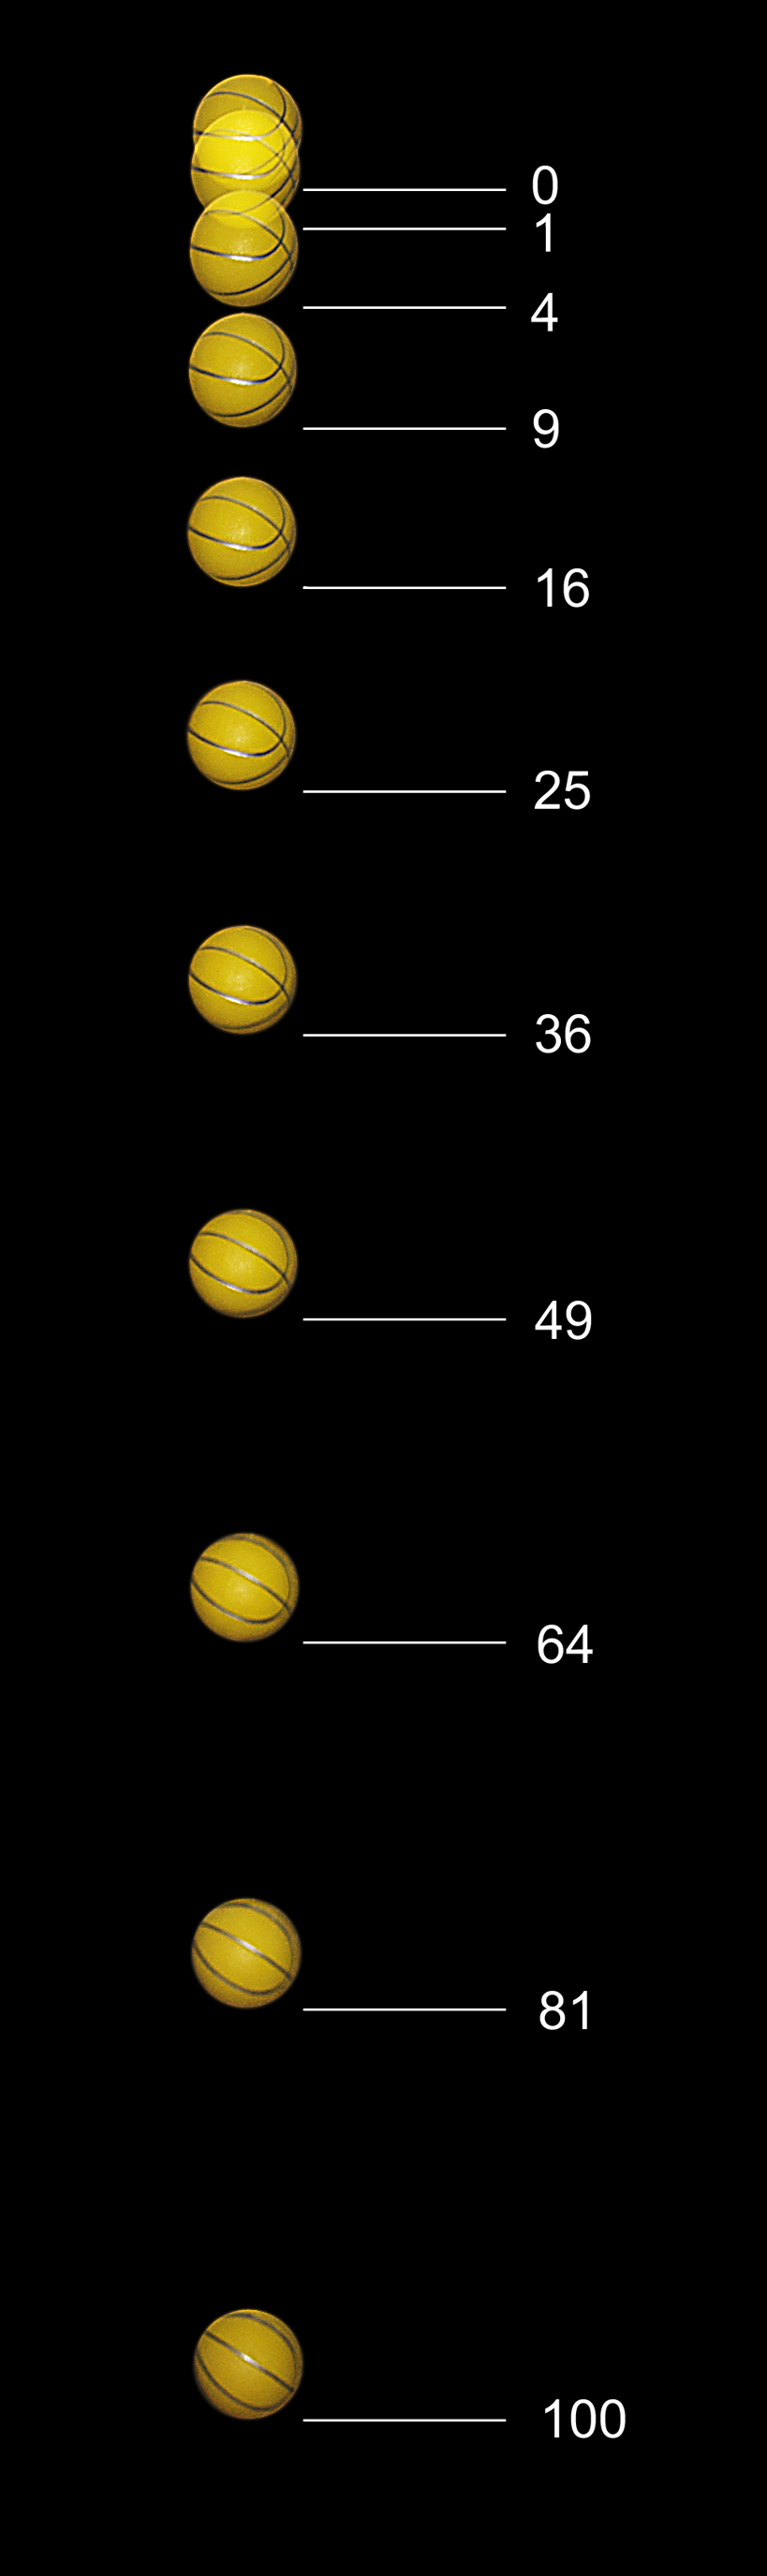
\includegraphics[width=0.15\textwidth]{00/fallingball.jpeg}
  };

\end{tikzpicture}}%
\only<1->{How can we use gravity to compute square roots?}

\only<2-3>{We know from physics}
\only<3->{
\begin{eqnarray*}
\only<3>{\ColorR{d} & = & \frac{1}{2} a \ColorG{t}^{2} \\}
\only<4->{\ColorG{t} & = & \sqrt{\frac{2\ColorR{d}}{a}}}
\end{eqnarray*}}
\only<5->{To compute $\sqrt{n}$, we just need to drop a ball from height $\ColorR{d}=\frac{an}{2}$ and measure the time for the ball to hit the ground.}
\only<6->{
\MedSkip{}
Example:
\begin{eqnarray*}
a & = & 9.8 \mbox{ m/$s^2$} \\
n & = & 81 \\
\ColorR{d} & = & an / 2 = 369.9 \mbox{ meters}
\end{eqnarray*}
Takes 9 seconds to drop}
\end{frame}

\begin{frame}{Using DNA to solve Traveling Salesperson\LinkArrow{https://www.jyi.org/2005-september/2005/9/7/fear-not-traveling-salesmen-dna-computing-is-here-to-save-the-day}}{Uses biophysical properties of ligation and electrophoresis}
    
\begin{columns}
    \begin{column}{0.5\textwidth}
        \begin{itemize}
            \item<1-> Each city is represented by a strand of DNA, with a unique first and last part.
            \item<2-> The strand of one city can ligate (attach) to the strand of an adjacent city, thus extending the path.
            \item<3-> These strands of DNA can be sorted by length using \href{https://en.wikipedia.org/wiki/Gel_electrophoresis}{electrophoresis}, with the shortest acceptable strand encoding the solution.
        \end{itemize}
 
    \end{column}
    \begin{column}{0.5\textwidth}  %%<--- here
     \begin{center}
        \vskip -2.5em
        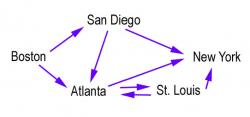
\includegraphics[width=0.7\textwidth]{00/map.jpeg}
     \end{center}
     \only<1->{
        \Vskip{-2em}
        \begin{tabular}{lcl}
            San Diego & = & \texttt{TTG AAA} \\
            Atlanta   & = & \texttt{TTT CTC}
        \end{tabular}
     }
     \only<2->{
        \MedSkip{}
        Possible ligation:
        
        \begin{tabular}{lll}
            \texttt{TTG} & \texttt{AAA} \\
               &  \texttt{TTT} & \texttt{CTC}
        \end{tabular}
     }
     
     \only<3->{
        \MedSkip{}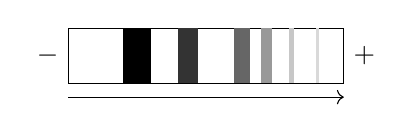
\begin{tikzpicture}[scale=0.7]
              \draw (0,0) rectangle(5,1);
              \node at (0,0.5) [left] {$-$};
              \node at (5,0.5) [right] {$+$};
              \draw[->] (0,-0.25) -- (5,-0.25);
              \fill[color=black!100!white] (1,0) rectangle(1.5,1);
              \fill[color=black!80!white] (2,0) rectangle(2.35,1);
              \fill[color=black!60!white] (3,0) rectangle(3.3,1);
              \fill[color=black!40!white] (3.5,0) rectangle(3.7,1);
              \fill[color=black!22!white] (4,0) rectangle(4.1,1);
              \fill[color=black!15!white] (4.5,0) rectangle (4.55,1);
        \end{tikzpicture}
     }
    \end{column}
\end{columns}

\end{frame}

\begin{frame}{Quantum effect}{Warning:  This material may be mind blowing}
\begin{itemize}
    \item Small particles such as electrons and photons live a very strange existence.
    \item We lack experience or even adequate language to understand and express how they behave.
    \item However, \href{https://en.wikipedia.org/wiki/Quantum_mechanics}{quantum mechanics} has been extraordinarily successful in predicting the outcomes of quantum events.
    \item Einstein did not (want to) believe that (his own) quantum theories were complete.\LinkArrow{https://en.wikipedia.org/wiki/Bohr-Einstein_debates}
\end{itemize}
\only<2->{
\begin{description}
    \item[Einstein:]  God does not play dice with the universe.
    \item[Bohr:] Don't tell God what to do with God's dice!
\end{description}}

\only<3->{\alert{
We can use quantum effects to compute interesting results.   In this course, we look at various problems and develop solutions based on quantum effects.}}

\end{frame}

\begin{frame}{Aside: physics theories}{What should they do for us?}
\begin{description}
    \item[predict outcomes]  The theory suffices when it predicts experimental results.  
    \begin{itemize}
        \item \href{https://en.wikipedia.org/wiki/Richard_Feynman}{Feynman} allegedly said \Quote{Shut up and calculate!}
        \item Perhaps he didn't say that. \LinkArrow{https://physicstoday.scitation.org/doi/10.1063/1.1768652}
        \item Maybe we should calculate but not be silent \LinkArrow{https://aeon.co/essays/shut-up-and-calculate-does-a-disservice-to-quantum-mechanics}
    \end{itemize}
    \item[explain stuff]  The theory should illuminate \emph{how} things work?
    \begin{itemize}
        \item What are the underlying mechanisms at work?
        \item What does this tell us about our world, how it was constructed, how it functions?
    \end{itemize}
\end{description}
This is an ongoing debate in physics.  We run into this problem studying how a ball flies through the air.  We can predict where it lands, but we cannot explain how gravity really works. 
\end{frame}
\begin{frame}{What are those quantum effects of interest to us?}{Superposition, interference, entanglement}
\begin{description}
    \item[Superposition:]  \only<1->{A quantum bit isn't necessarily in one state or another, but can be in a \emph{superposition} of states.  \only<1-3>{For example, consider a bucket of $r$~red and~$b$ blue marbles.  Until you draw a marble, the outcome is characterized as $r/(r+b)$ red $+$ $b/(r+b)$ blue.}}
    \only<2-3>{
    
    Once you draw from the bucket, that outcome has \emph{collapsed} to either fully red or fully blue.  
    
    Moreover, if you look at that drawn marble any number of times, it stays the same color.}
    
    
    \OnlyRemark{3}{
    In a quantum system, we can easily create the superposition of \emph{all} possible inputs to a function.}
    \only<4->{
    \item[Interference:]  In the superposition, we can influence the probability, up or down, of seeing a particular outcome using \emph{interference}.
    
    \only<4>{The effect here is akin to waves in a pool of water.   Based on their relative phases, two waves can pass through each other and either amplify or cancel each other.
    \Remark{We will use interference to emphasize the outcomes we wish to see.}
    }
    
    }
    \only<5->{
    \item[Entanglement:]  When two quantum bits are \emph{entangled}, their measurement outcomes are correlated, even if those outcomes are random.
    
    This is the most strange and useful property of quantum systems.  
    
    We will show that there is no information shared by such quantum bits that explains that behavior.
    
    
    }
\end{description}
\only<6>{\Example{We can entangle two quantum bits so that they randomly both measure either \True{} or \False{}, even if they are separated by light years from each other.}}

\only<7>{
\MedSkip{}Why do we care?  Harnessing these quantum effects allows us to solve some interesting problems in mere seconds that would take billions of years to solve on a classical computer.}
    
\end{frame}

\section{Logistics}

\begin{frame}{Course overview and logistics}{You are responsible for this knowledge}
The information is contained on this semester's \href{https://wustl.instructure.com/courses/80191/pages/overview-grading-academic-integrity?module_item_id=1145453}{canvas page}
\begin{itemize}
    \item Lecture
    \item Homework
    \item Exams
    \item Group work
    \item Academic integrity
    \item How to get help
\end{itemize}
\end{frame}

\begin{frame}{Course outline}{Subject to change}
\Vskip{-4em}\TwoColumns{%
\begin{enumerate}
    \item Introduction and background
    \item Reversible computations
    \item Computational complexity
    \item The physics
    \item Quantum systems
    \item Single qubit
    \item Universal quantum gates
    \item Elitzur--Vaidman bomb
    \item Beyond one qubit
    \item No-cloning theorem
    
\end{enumerate}
}{%
\begin{enumerate}
    \setcounter{enumi}{10}
    \item Quantum teleportation
    \item Quantum advantage
    \item Deutsch's problem
    \item Phase kickback trick
    \item Deutsch--Jozsa problem
    \item Simon's problem
    \item Bernstein--Vazirani problem
    \item Phase estimation
    \item Quantum Fourier
    \item Shor's algorithm
    \item Grover's algorithm
\end{enumerate}
}
    
\end{frame}

\end{document}
